\documentclass[10pt,letterpaper]{article}\usepackage[]{graphicx}\usepackage[]{color}
%% maxwidth is the original width if it is less than linewidth
%% otherwise use linewidth (to make sure the graphics do not exceed the margin)
\makeatletter
\def\maxwidth{ %
  \ifdim\Gin@nat@width>\linewidth
    \linewidth
  \else
    \Gin@nat@width
  \fi
}
\makeatother

\definecolor{fgcolor}{rgb}{0.345, 0.345, 0.345}
\newcommand{\hlnum}[1]{\textcolor[rgb]{0.686,0.059,0.569}{#1}}%
\newcommand{\hlstr}[1]{\textcolor[rgb]{0.192,0.494,0.8}{#1}}%
\newcommand{\hlcom}[1]{\textcolor[rgb]{0.678,0.584,0.686}{\textit{#1}}}%
\newcommand{\hlopt}[1]{\textcolor[rgb]{0,0,0}{#1}}%
\newcommand{\hlstd}[1]{\textcolor[rgb]{0.345,0.345,0.345}{#1}}%
\newcommand{\hlkwa}[1]{\textcolor[rgb]{0.161,0.373,0.58}{\textbf{#1}}}%
\newcommand{\hlkwb}[1]{\textcolor[rgb]{0.69,0.353,0.396}{#1}}%
\newcommand{\hlkwc}[1]{\textcolor[rgb]{0.333,0.667,0.333}{#1}}%
\newcommand{\hlkwd}[1]{\textcolor[rgb]{0.737,0.353,0.396}{\textbf{#1}}}%
\let\hlipl\hlkwb

\usepackage{framed}
\makeatletter
\newenvironment{kframe}{%
 \def\at@end@of@kframe{}%
 \ifinner\ifhmode%
  \def\at@end@of@kframe{\end{minipage}}%
  \begin{minipage}{\columnwidth}%
 \fi\fi%
 \def\FrameCommand##1{\hskip\@totalleftmargin \hskip-\fboxsep
 \colorbox{shadecolor}{##1}\hskip-\fboxsep
     % There is no \\@totalrightmargin, so:
     \hskip-\linewidth \hskip-\@totalleftmargin \hskip\columnwidth}%
 \MakeFramed {\advance\hsize-\width
   \@totalleftmargin\z@ \linewidth\hsize
   \@setminipage}}%
 {\par\unskip\endMakeFramed%
 \at@end@of@kframe}
\makeatother

\definecolor{shadecolor}{rgb}{.97, .97, .97}
\definecolor{messagecolor}{rgb}{0, 0, 0}
\definecolor{warningcolor}{rgb}{1, 0, 1}
\definecolor{errorcolor}{rgb}{1, 0, 0}
\newenvironment{knitrout}{}{} % an empty environment to be redefined in TeX

\usepackage{alltt}
\usepackage[top=0.85in,left=1.75in,footskip=0.75in]{geometry}

% amsmath and amssymb packages, useful for mathematical formulas and symbols
\usepackage{amsmath,amssymb}

% Use adjustwidth environment to exceed column width (see example table in text)
\usepackage{changepage}

% Use Unicode characters when possible
\usepackage[utf8x]{inputenc}

% textcomp package and marvosym package for additional characters
\usepackage{textcomp,marvosym}

% cite package, to clean up citations in the main text. Do not remove.
\usepackage{cite}

% Use nameref to cite supporting information files (see Supporting Information section for more info)
\usepackage{nameref,hyperref}

% line numbers
\usepackage[right]{lineno}

% ligatures disabled
\usepackage{microtype}
\DisableLigatures[f]{encoding = *, family = * }

% color can be used to apply background shading to table cells only
\usepackage[table]{xcolor}

% array package and thick rules for tables
\usepackage{array}

% highlighting
\usepackage{soul}

% bold math symbols package
\usepackage{bm}

% nice figures and captions
\usepackage{graphicx}

% diagrams or complicated equations
\usepackage{tikz}

% vertical and horizontal dashed lines
%\usepackage{arydshln}

%\usepackage{setspace}

%\usepackage{floatflt}
%\usepackage{nonfloat}
\usepackage{float}
%\usepackage{wrapfig}
\usepackage{longtable,booktabs}
\usepackage{tabu}

\usepackage{harpoon}
\usepackage{fdsymbol}

%\renewcommand{\arraystretch}{1.2}
%\setlength{\tabcolsep}{12pt}

% create "+" rule type for thick vertical lines
\newcolumntype{+}{!{\vrule width 2pt}}

% create \thickcline for thick horizontal lines of variable length
\newlength\savedwidth
\newcommand\thickcline[1]{%
  \noalign{\global\savedwidth\arrayrulewidth\global\arrayrulewidth 2pt}%
  \cline{#1}%
  \noalign{\vskip\arrayrulewidth}%
  \noalign{\global\arrayrulewidth\savedwidth}%
}

% \thickhline command for thick horizontal lines that span the table
\newcommand\thickhline{\noalign{\global\savedwidth\arrayrulewidth\global\arrayrulewidth 2pt}%
\hline
\noalign{\global\arrayrulewidth\savedwidth}}


% Remove comment for double spacing
%\usepackage{setspace} 
%\doublespacing

% Text layout
% \raggedright
\setlength{\parindent}{0.5cm}
\textwidth 5.25in 
\textheight 8.75in

% Bold the 'Figure #' in the caption and separate it from the title/caption with a period
% Captions will be left justified
\usepackage[aboveskip=1pt,labelfont=bf,labelsep=period,justification=raggedright,singlelinecheck=off]{caption}
\renewcommand{\figurename}{Fig}

% Use the PLoS provided BiBTeX style
%\bibliographystyle{plos2015}


% Remove brackets from numbering in List of References
\makeatletter
\renewcommand{\@biblabel}[1]{\quad#1.}
\makeatother

% define theorem and definition environments commands
\newtheorem{theorem}{Theorem}[section]
\newtheorem{definition}{Definition}[section]

% Header and Footer with logo
\usepackage{lastpage,fancyhdr,graphicx}
\usepackage{epstopdf}
%\pagestyle{myheadings}
\pagestyle{fancy}
\fancyhf{}
%\setlength{\headheight}{27.023pt}
%\lhead{\includegraphics[width=2.0in]{PLOS-submission.eps}}
\rfoot{\thepage/\pageref{LastPage}}
\renewcommand{\headrulewidth}{0pt}
\renewcommand{\footrule}{\hrule height 2pt \vspace{2mm}}
\fancyheadoffset[L]{2.25in}
% \fancyfootoffset[L]{1.25in}
\lfoot{\today}


\restylefloat{figure}


%% Include all macros below

\newcommand{\lorem}{{\bf LOREM}}
\newcommand{\ipsum}{{\bf IPSUM}}

\def\lf{\left\lfloor}   
\def\rf{\right\rfloor}

\def\ri{R_i}
\def\rj{R_j}
\def\kmi{k_{M_i}}
\def\khi{k_{H_i}}
\def\hji{H_{j_i}}
\def\ma{\overline{M}_a}
\def\ha{\overline{H}_a}
\def\mnu{M_\nu}
\def\hnu{H_\nu}
\def\myd{\text{diff}}
\def\ka{\bar{k}_\alpha}
\def\mji{M_{j_i}}

%% END MACROS SECTION
\IfFileExists{upquote.sty}{\usepackage{upquote}}{}
\begin{document}
\vspace*{0.2in}

% Title must be 250 characters or less.
% \begin{flushleft}
{\Large
\textbf\newline{Novel metrics and application of nearest-neighbor feature selection for comparing resting-state fMRI brain atlases} % Please use "sentence case" for title and headings (capitalize only the first word in a title (or heading), the first word in a subtitle (or subheading), and any proper nouns).
}
%\newline
% Insert author names, affiliations and corresponding author email (do not include titles, positions, or degrees).
\begin{center}
  \begin{tabular}{l}
  Bryan A. Dawkins$^{\text{1}}$, Rayus Kuplicki$^{\text{2}}$, Trang T. Le$^{\text{3}}$, Alejandro A. Hernandez$^{\text{1}}$, \\
  and Brett A. McKinney$^{\text{1,4,}*}$ \\
  $^{\text{1}}$Department of Mathematics, University of Tulsa, Tulsa, OK 74104, USA \\
  $^{\text{2}}$Laureate Institute for Brain Research, Tulsa, OK 74136, USA \\
  $^{\text{3}}$Department of Biostatistics, Epidemiology and Informatics, University of \\
  \hphantom{2}Pennsylvania, Philadelphia, PA 19104 \\
  $^{\text{4}}$Tandy School of Computer Science, University of Tulsa, Tulsa, OK 74104, USA\\
  $*$Correspondence: brett.mckinney@gmail.com
  \end{tabular}
\end{center}


% \end{flushleft}
% Please keep the abstract below 300 words
\section*{Abstract}
Resting-state functional connectivity MRI (rs-fMRI) data consists of correlation matrices, where correlations are computed between the time series from brain Regions of Interest (ROIs). There are many different parcellations of the human brain into collections of ROIs. These parcellations, or atlases, can be used in case-control studies in order to understand and accurately classify subject phenotypes. We present new metrics for nearest-neighbor distance-based feature selection at the ROI level. Using our new metrics, we apply a novel nearest-neighbor feature selection algorithm to calculate relative importance of ROIs for classification of a binary outcome including major depression and healthy controls in two existing brain atlases. We use integer programming to derive a mapping between brain atlases to determine spatially similar ROIs. With ROI importance scores and spatial similarity between atlases, we present a novel modality for the comparison of brain atlases and the selection of ROIs relevant to major depression.
\linenumbers

%\doublespacing
\section{Background}
Resting-state fMRI data exists in high dimensions and has many sources of noise, such as physiological or motion related~\cite{caballero2017}. Feature selection is typically done with the purpose of determining brain regions of interest (ROIs) that accurately discriminate between cases and controls in order to understand a particular phenotype. The data consists of pairwise ROI-ROI correlations, where each ROI is a time series measuring brain activity in a particular region or regions of the brain while a subject is not performing a task. A typical data set consists of $m$ subject-specific correlation matrices of dimension $p \times p$, where the pairwise correlations are computed between $p$ ROI time series with respect to a particular brain atlas. 

Nearest-neighbor distance-based feature selection in rs-fMRI data has been performed using the private evaporative cooling method, which used pairwise ROI-ROI correlations as predictors of a particular phenotype~\cite{le17}. However, nearest-neighbor feature selection algorithms have not been applied at the ROI level to assess the relative importance of ROIs for a given phenotype. To address this, we have previously proposed a new distance metric that allows us to compute the importance of individual ROIs using a nearest-neighbor distance-based approach (cite theoretical paper). We use this new distance metric with a novel nearest-neighbor feature selection algorithm called Nearest-neighbor Projected Distance Regression (NPDR) in order to compute ROI importance and the corresponding pseudo P values~\cite{npdr}. Our analysis is done on subject rs-fMRI correlation matrices generated by two well known brain atlases with spherical~\cite{power2011} and anatomically shaped~\cite{shen2013} ROIs, to which we refer as Power and Shen atlases, respectively. Cross sections through each atlas were visualized (Fig.~\ref{fig:power_shen_unmapped}) using the Analysis of Functional NeuroImages (AFNI) software~\cite{cox1996}.

\vspace{0.25cm}

% trim=left botm right top
%\begin{figure}[h!]\label{fig:jaccard}
{\centering
	\begin{minipage}[c]{0.55\textwidth}
		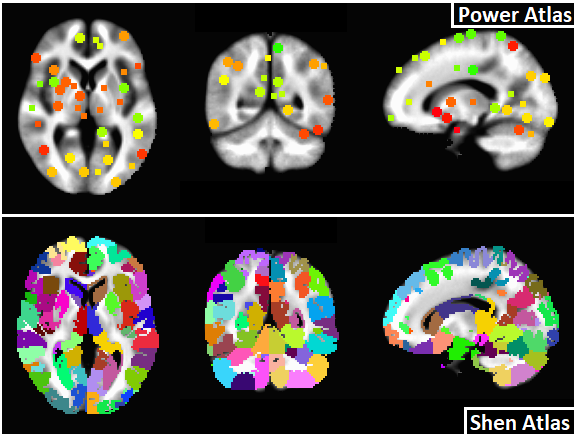
\includegraphics[width=1\textwidth,clip,trim=0cm 0cm 0cm 0.0cm]{power_shen_montage2.png}
	\end{minipage}\hfill
	\begin{minipage}[c]{0.43\textwidth}
		\captionsetup{type=figure}\captionof{figure}{Two-dimensional slices through Power~\cite{power2011} and Shen~\cite{shen2013} atlas ROIs. Slices are shown at the same locations in each atlas for the three different orientiations. Atlases are in MNI space~\cite{collins1994} so that voxel and ROI locations are comparable between them. Each atlas is labeled by the first author of the manuscripts in which they were introduced~\cite{power2011,shen2013}.}\label{fig:power_shen_unmapped}
\end{minipage}}
%\end{figure}

\vspace{0.25cm}

In order to make spatial comparisons between any pair of brain atlases, we first compute a distance matrix containing all pairwise distances between the different collections of atlas ROIs. Distances are defined based on a set dissimilarity metric that accounts for differences in voxel collections between pairs of ROIs. In a particular coordinate system, voxels have well defined three-dimensional locations in a given brain atlas. As long as two different atlases are in the same coordinate system, we can compare voxel membership between opposing atlas ROIs. We use an integer program that defines the standard Assignment Problem (AP) to find the one-to-one mapping between the two sets of atlas ROIs~\cite{pentico2007}. The collection of all mapped ROIs gives the closest spatial analogy between the two atlases, which tells us the closest relationship between the two sets of ROIs from different atlases. The collection of unmapped ROIs gives an indication of spatial uniqueness in the two atlases, respectively. All ROIs can be further mapped to a well defined anatomical region of the brain, which allows us to point out potential targets for better understanding the phenotype of interest.

Our spatial mapping between atlases and relative importance scores for ROIs in each respective atlas provides a way to combine relevant and distinct aspects of each brain atlas into a new parcellation. This new atlas includes important ROIs that are in the optimal one-to-one mapping from the solution to the assignment problem and any important unmapped ROIs from each atlas. Spatial overlap and attribute importance can serve as a useful tool for other researchers to compare, contrast, and combine two atlases. In particular, our results show how one might choose either of the two atlases to study the phenotype of interest we are considering in this work.

\section{Methods}
In this section, we first describe real rs-fMRI data generated from healthy controls (HC) and subjects with major depressive disorder (MDD), eating disorder (ED), substance abuse (SA), or anxiety disorder (AD). Using integer programming, we then derive a one-to-one mapping between the ROIs in two brain atlases used to generate the real data mentioned previously. Finally, we use our new distance metric for rs-fMRI data, along with NPDR, to compute importance scores for ROIs in each atlas from the real data.

\subsection{Real rs-fMRI data}
% need to get with Rayus to discuss the details on what the data is, how it was processed,
% more demographics info for subjects, and anything else that might be important
This is where we describe the LIBR data.

\subsection{Spatial overlap between brain atlases}
Let $R_A$ and $R_B$ represent regions of interest (ROIs) in atlases $A$ and $B$, respectively. We assume that atlases $A$ and $B$ are in the same coordinate space. Since $R_A$ and $R_B$ are just collections of voxels that have well defined three-dimensional coordinates within an atlas, the spatial overlap between $R_A$ and $R_B$ can be defined as the set intersection between the two ROIs. Spatial dissimilarity between $R_A$ and $R_B$ can be computed with the Jaccard metric, which is given by the following
%
\begin{equation}\label{eq:jaccard}
\text{d}^\text{J}(R_A,R_B) = \frac{|R_A \cup R_B - R_A \cap R_B|}{|R_A \cup R_B|},
\end{equation}
%
where the ($-$) sign denotes set complement and $|\cdot|$ represents set cardinality. If the intersection $R_A \cap R_B$ is empty, then the two ROIs do not share any voxels and the Jaccard distance (Eq.~\ref{eq:jaccard}) between them is 1. On the other hand, the Jaccard distance is 0 if the union $R_A \cup R_B$ and intersection $R_A \cap R_B$ are the same sets, which means the two ROIs have exactly the same voxels. All other possible Jaccard distances between $R_A$ and $R_B$ are strictly within $(0,1)$. Hence, the Jaccard metric is contained within $[0,1]$. The reason for division by $|R_A \cup R_B|$ in the denominator of the Jaccard metric (Eq.~\ref{eq:jaccard}) is specifically to normalized the distance to be within $[0,1]$. Otherwise, this distance between two ROIs would be affected by the cardinalities of $R_A$ and $R_B$, respectively. The Jaccard metric is intuitive in this context because ROIs are not just points in space, but rather they can have irregular three-dimensional shapes. Therefore, a Euclidean metric that gives the straight-line distance between two points does not necessarily indicate `closeness' between two ROIs. It is possible to compute the Euclidean distance between the centroids of two ROIs, but the ROIs may not share many voxels due to their potentially irregular shapes. Therefore, it is more informative to use a distance metric that uses set operations like the Jaccard metric (Eq.~\ref{eq:jaccard}). We show an example (Fig.~\ref{fig:jaccard}) of the Jaccard distance between ROIs $R_A$ and $R_B$ that contain $n_1$ and $n_2$ voxels, respectively. 

\vspace{0.25cm}

% trim=left botm right top
%\begin{figure}[h!]\label{fig:jaccard}
	{\centering
	\begin{minipage}[c]{0.55\textwidth}
	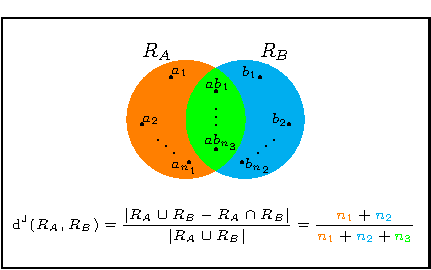
\includegraphics[width=1\textwidth,clip,trim=0cm 0cm 0cm 0.26cm]{venn_diagram.pdf}
	\end{minipage}\hfill
	\begin{minipage}[c]{0.43\textwidth}
	\captionsetup{type=figure}\captionof{figure}{Example computation of Jaccard distance between ROIs $R_A$ and $R_B$ from two atlases $A$ and $B$, respectively. There are $n_1$, $n_2$, $n_3$ voxels in $R_A$ only, $R_B$ only, and both $R_A$ and $R_B$, respectively. The numerator gives the number of voxels unique to $R_A$ ($n_1$) plus the number of voxels unique to $R_B$ ($n_2$). The denominator contains the total number of voxels in $R_A$ or $R_B$.}\label{fig:jaccard}
	\end{minipage}}
%\end{figure}

\vspace{0.25cm}

Each ROI in atlas $A$ may overlap many different ROIs in atlas $B$. On the other hand, some ROIs in $A$ may not overlap any ROIs in $B$. Furthermore, it is likely that $A$ and $B$ contain different numbers of ROIs. If we want to compute a minimum distance one-to-one mapping between the atlases, it is possible that some ROIs in $A$ will not have a mapped partner in $B$. In order to efficiently compute this atlas-atlas mapping, we formulate this task as a standard Assignment Problem~\cite{pentico2007}, which has a very concise definition (Fig.~\ref{fig:assignment_problem}).

\vspace{0.25cm}

%\begin{figure}[h!]\label{fig:jaccard}
{\centering
	\begin{minipage}[c]{0.55\textwidth}
		\framebox{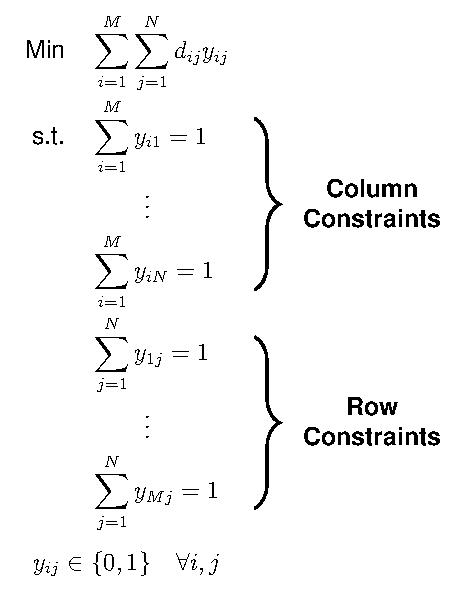
\includegraphics[width=1\textwidth,clip,trim=0cm 0cm 0cm 0.26cm]{assignment_problem_equations.pdf}}
	\end{minipage}\hfill
	\begin{minipage}[c]{0.4\textwidth}
		\captionsetup{type=figure}\captionof{figure}{Assignment problem mathematical definition. The assignment matrix $Y$ is binary, where $y_{ij}=0$ if nodes $i$ and $j$ are assigned to each other and 0 otherwise. The distance matrix $D$ between all nodes is computed to assign costs to arcs (or edges) between nodes. The distance between nodes $i$ and $j$ is denoted by $d_{ij}$. Therefore, the objective function is the sum of all pairwise distances in the collection of assigned arcs. the column and row constraints dictate that each node is connected to exactly one and only one other node.}\label{fig:assignment_problem}
\end{minipage}}
%\end{figure}

\vspace{0.25cm}

The objective function is the sum over all pairwise distances between nodes included in the mapping, where inclusion is determined by the binary solution matrix $Y$ that has the following definition
%
\begin{equation}\label{eq:assignment_sol}
y_{ij}=\begin{cases}
1 & \text{nodes } i \text{ and } j \text{ connected,} \\
0 & \text{otherwise.}
\end{cases}
\end{equation}

Each row and each column of $Y$ has a sum-to-one constraint, which means that each node in one collection is connected to exactly one other node in another disjoint collection. This problem assumes that the order (or size) of each collection is equal ($M=N$ in Fig.~\ref{fig:assignment_problem}), so that a one-to-one assignment is possible. In the context of brain atlases, we will satisfy this requirement by adding artificial variables to our solution matrix $Y$. Pairwise distances between actual ROIs in a brain atlas and an artificial variable will be given a large constant value, so that ROIs in atlas $A$ will preferentially map to another ROI in $B$ if a mapping is possible. Absent the possibility of a mapping, an ROI will map to an artificial variable, which implies that this particular ROI goes unmapped in our unconstrained solution. We show a diagram of atlas-atlas mapping (Fig.~\ref{fig:assignment_atlases}) that depicts ROIs as nodes and possible mappings as dashed lines between nodes in atlases $A$ and $B$. Each possible mapping has a distance ($d_{ij}$) associated with its inclusion in the solution matrix $Y$. The solution is ultimately found by choosing connections (solid lines) between atlas ROIs so that each ROI in $A$ is connected to exactly one ROI in $B$, which simultaneously minimizes the sum of all distances in the mapping. We also show how this mapping might look with respect to the actual brain atlases we consider in this manuscript (Fig.~\ref{fig:power_shen_mapped}). We have taken the unlabeled two-dimensional slices through each atlas (Fig.~\ref{fig:power_shen_unmapped}) and assigned ROIs to each other based on similar location. Each of the atlases are in the Montreal Neurological Institute (MNI) coordinate space~\cite{collins1994}, which allows us to compare the two atlases.

\begin{figure}[h!]
	\centering
	\framebox{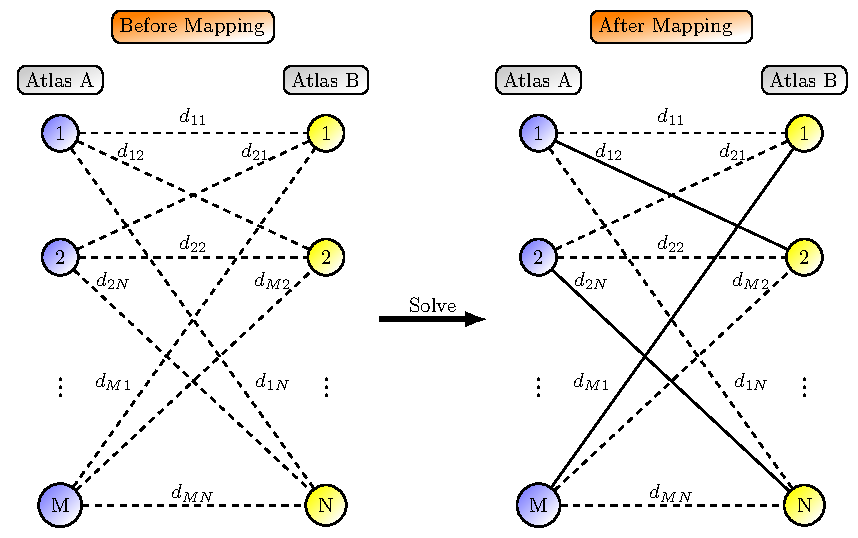
\includegraphics[width=0.98\textwidth]{assignment_diagram.pdf}}
	\caption{Assignment problem for brain atlas ROI-ROI mapping. Before the minimum distance pairwise mapping is found, all possible pairwise mappings are possible (dashed lines). Each ROI in atlas $A$ must have exactly one partner in atlas $B$. After mapping, the minimum distance pairs are selected to give a one-to-one correspondence between ROIs (solid lines).}\label{fig:assignment_atlases}
\end{figure}

% trim=left botm right top
%\begin{figure}[h!]\label{fig:jaccard}
{\centering
	\begin{minipage}[c]{0.55\textwidth}
		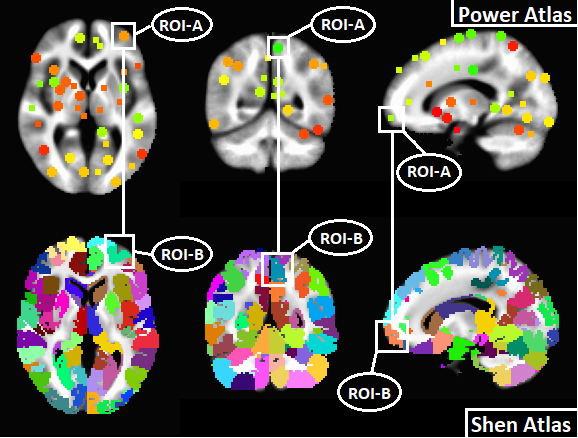
\includegraphics[width=1\textwidth,clip,trim=0cm 0cm 0cm 0.0cm]{power_shen_montage_mapped.png}
	\end{minipage}\hfill
	\begin{minipage}[c]{0.43\textwidth}
		\captionsetup{type=figure}\captionof{figure}{Visualization of mapping between Power and Shen atlas ROIs~\cite{power2011,shen2013}. ROIs that are in similar locations are potential partners in the resulting mapping from solving the assignment problem (Fig.~\ref{fig:assignment_problem}). The Power atlas~\cite{power2011} is labeled atlas $A$, while the Shen atlas is labeled $B$.}\label{fig:power_shen_mapped}
\end{minipage}}
%\end{figure}

\vspace{0.25cm}

\subsection{Relative importance of ROIs}

We load all subject-level resting-state fMRI (rs-fMRI) correlation matrices into a single matrix for our analysis (Fig.~\ref{fig:rs-fMRI_matrix}). Each column represents a single instance $i \in \mathcal{I}$ and each consecutive collection of $p-1$ rows represents a single ROI $a \in \mathcal{A}$. We apply a Fisher r-to-z transform to all pairwise correlations and then standardize so that each column is approximately standard normally distributed ($\mathcal{N}(0,1)$).

\bigskip

\begin{minipage}[c]{0.7\textwidth}\hspace{-0.6cm}
	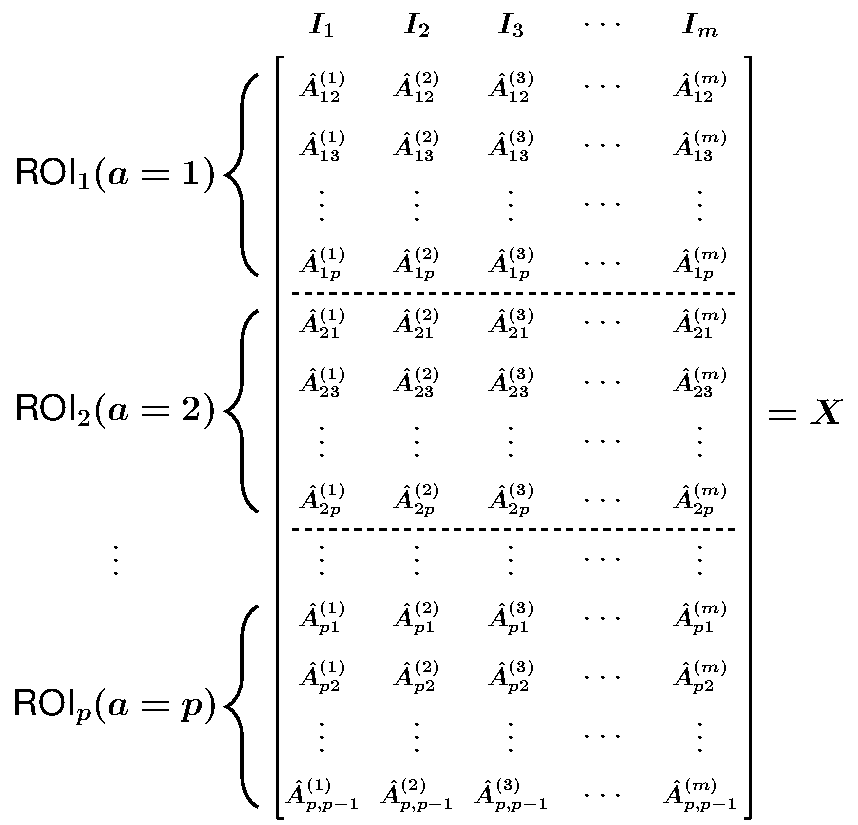
\includegraphics[width=0.95\textwidth]{fig5_rs_fmri_all_instance_matrix.pdf}
\end{minipage}\hspace{-0.8cm}
\begin{minipage}[c]{0.3\textwidth}
	\captionsetup{type=figure}\captionof{figure}{Organization based on brain regions of interest (ROIs) of resting-state fMRI correlation dataset consisting of transformed correlation matrices for $m$ subjects. Each column corresponds to an instance (or subject) $I_j$ and each subset of rows corresponds to the correlations for an ROI attribute ($p$ sets). The notation $\hat{A}^{(j)}_{ak}$ represents the r-to-z transformed correlation between attributes (ROIs) $a$ and $k \neq a$ for instance $j$.}\label{fig:rs-fMRI_matrix}
\end{minipage}

\bigskip

We determine attribute importance using Nearest-neighbor Projected Distance Regression (NPDR)~\cite{npdr}, which is a novel nearest-neighbor feature selection method that builds upon Relief-Based Algorithms (RBAs)~\cite{robnik2003,urbanowicz17}. For binary response variables, like case-control outcomes, NPDR computes a standardized beta coefficient for a generalized linear model (GLM) (Fig.~\ref{fig:npdr_finished}). The argument to the logit function is $\text{p}^\text{miss}_{ij}$, which is the probability that instances $i,j \in \mathcal{I}$ are in different phenotype classes. This argument models the binary outcome diff, which is given by the following
%
\begin{equation}\label{eq:diff_outcome}
\text{d}^\text{miss}_{ij}(\overrightharpoon{y})=\begin{cases}
0 & y_i = y_j, \\
1 & \text{else}.
\end{cases}
\end{equation}

For each coefficient $\beta_a$, a significant adjusted pseudo P value implies that the null hypothesis ($\beta_a \leq 0$) is rejected. The alternative hypothesis ($\beta_a > 0$) implies that the particular attribute $a \in \mathcal{A}$ may be important for classification.

In order to compute distances, we previously introduced a metric for time series-correlation based (ts-corr) data like rs-fMRI~(cite BoD theoretical). The one-dimensional projection (diff) onto a single ROI is define as follows
%
\begin{equation}\label{eq:diff_rs-fMRI}
\text{d}^\text{ROI}_{ij}(a) = \sum_{k \neq a}\bigl|A^{(i)}_{ka} - A^{(j)}_{ka}\bigr|,
\end{equation}
%
where $A^{(i)}_{ak}$ and $A^{(j)}_{ak}$ are the correlations between ROI $a$ and ROI $k$ for instances $i,j \in \mathcal{I}$, respectively. With this rs-fMRI diff, we define the pairwise distance between two instances $i,j \in \mathcal{I}$ as follows
%
\begin{equation}\label{eq:D_rs-fMRI}
D^\text{fMRI}_{ij} = \sum_{a \in \mathcal{A}} \text{d}^\text{ROI}_{ij}(a).
\end{equation}

Using our attribute diff (Eq.~\ref{eq:diff_rs-fMRI}), we compute standardized beta coefficients of the generalized linear model given by
%
\begin{equation}\label{eq:glm_roi}
\text{logit}\left(\text{p}^\text{miss}_{ij}\right) = \beta_0 + \beta_a \text{d}^\text{ROI}_{ij}(a) + \epsilon_{ij}, \quad \forall(i,j) \in \mathcal{N}(k),
\end{equation}
%
which is the GLM that NPDR uses to compute standardized beta coefficients for binary outcomes with $\text{d}_{ij}(a)$ (Fig.~\ref{fig:npdr_finished}) replaced by our diff for ROIs $\text{d}^\text{ROI}_{ij}(a)$ (Eq.~\ref{eq:diff_rs-fMRI}). The collection of all neighbor ordered pairs is denoted by $\mathcal{N}(k)$. This set is a function of $k$ because we use a fixed-$k$ approach in NPDR to allow each attribute $a \in \mathcal{A}$ to have its own optimal value of $k$.

\begin{figure}[h!]
	\centering
	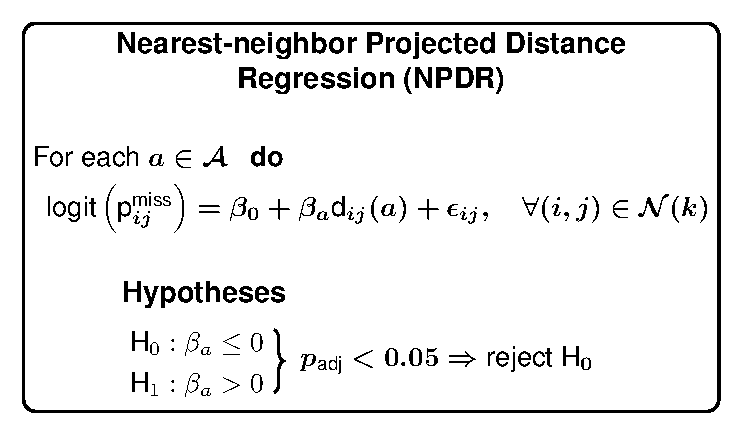
\includegraphics[width=0.85\textwidth]{npdr_finished_diagram.pdf}
	\caption{Nearest-neighbor Projected Distance Regression for binary response (case-control)~\cite{npdr}. For each attribute $a \in \mathcal{A}$, we compute standardized beta coefficients for a generalized linear model, where the predictors ($\text{d}_{ij}(a) = |X_{ia} - X_{ja}|$) are one-dimensional projected distances (diffs) with respect to a particular attribute. The argument $\text{p}^\text{miss}_{ij}$ is the probability that instances $i,j \in \mathcal{I}$ are in different phenotype classes. The logit function models the binary hit-miss phenotype projection (Eq.~\ref{eq:diff_outcome}). Significant adjusted pseudo P values ($p_\text{adj}$) lead to the rejection of the null hypothesis $\beta_a \leq 0$. The set $\mathcal{N}(k)$ is the collection of all neighbor ordered pairs such that each target instances neighborhood as exactly $k$ nearest neighbors.}\label{fig:npdr_finished}
\end{figure}

We employ an adaptive-$k$ algorithm called Gene-Wise Adaptive $k$ (GWAK) that was originally developed for gene expression data~\cite{mckinney13} to determine the optimal $k$ for each ROI in the two atlases we are analyzing. Although developed for gene expression data, this method can be used for other data types to which nearest-neighbor feature selection is applied. GWAK uses a greedy approach to optimize the relevance score for each attribute as a function of $k$ (Fig.~\ref{fig:gwak}). For each attribute $a \in \mathcal{A}$, a relevance score is computed for each value of $k=1,2,\dots,m-1$ using some nearest-neighbor feature selection algorithm. Each attribute is assigned the value of $k$ that maximizes its relevance score. For noise attributes, scores do not change significantly as a function of $k$. On the other hand, the scores of relevant attributes will change significantly as a function of $k$. This implies that GWAK maximizes the probability of detecting relevant attributes when nearest-neighbor feature selection is utilized. 

We have previously shown that cross-validation approaches for tuning $k$ to optimally select relevant features do not perform well in nearest-neighbor feature selection as compared to GWAK (cite simulation paper). This is due largely to the fact that cross-validation is optimizing test classification accuracy, which does not necessarily correlate with the relevance or quality of selected features. Partitioning data into training and test folds also limits the choice of $k$ because the training data has only a subset of available instances in the full data set. This partitioning may cause the selection of a suboptimal $k$ for a relevant attribute, which could be detrimental to the quality of selected features.

\begin{figure}[h!]
	\centering
	\framebox{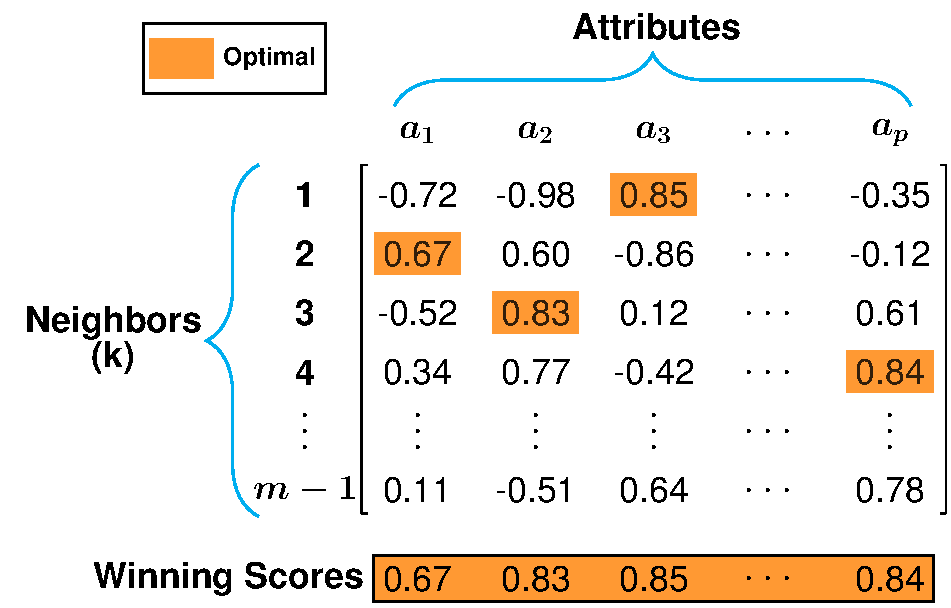
\includegraphics[width=0.8\textwidth]{feature_wise_opt_diagram3.pdf}}
	\caption{Feature-wise adaptive-$k$ method for choosing optimal values of $k$ in nearest-neighbor feature selection. For each attribute $a \in \mathcal{A}$ and each value of $k=1,2,\dots,m-1$, a score or weight is computed with a nearest-neighbor feature selection method like Relief-Based Algorithms (RBAs) or another similar method. Each feature is assigned the value of $k$ that maximizes its importance score. Winning scores are then sorted in decreasing order and some fraction of the top scoring attributes are chosen for further analysis. We use the adjusted pseudo P values from NPDR to filter out attributes that are determined irrelevant to the phenotype. With NPDR, attribute scores are simply the standardized beta coefficients computed for the corresponding GLM (Eq.~\ref{eq:glm_roi}).}\label{fig:gwak}
\end{figure}

\section{Results}
In this section, we first give a pairwise mapping between the Power and Shen brain atlases. We describe the process of solving for a minimum distance one-to-one mapping. We then show which ROIs in the two atlases are determined important by NPDR, which are partitioned by those that are mapped and unmapped. Finally, we demonstrate the validity of important ROIs by referencing other analyses that have produced similar results.

\subsection{Power and Shen atlas mapping}
Since there are 277 and 278 ROIs in Power and Shen atlases, respectively, we first compute a distance matrix $D$ that contains all pairwise distances between atlas ROIs. This gives us a $278 \times 277$ distance matrix to which we add a column of large numeric entries to represent distances from ROIs to an artificial variable. This makes the distance matrix square, which allows us to satisfy the one-to-one constraint of the Assignment Problem (Fig.~\ref{fig:assignment_problem}). We used the open source statistical computing software \textbf{\textsf{R}}~\cite{R}, which includes a package called \textsf{lpSolve}~\cite{lpsolve} for solving a variety of linear and integer programs. The \textsf{lpSolve} package contains a function \textsf{lp.assign()}, which simply takes a square distance matrix as input and produces solution matrix $Y$ and an objective function value as output. For distance matrices comparable in dimension to $D$, the function elapses only a few seconds in run time.

The solution matrix from \textsf{lp.assign()} has a total of 230 actual mapped pairs. Some of the entries in the solution matrix $Y$ are extraneous, which we define as one of the following: an ROI pair including an artificial variable, an ROI pair for which the Jaccard dissimilarity is maximal (e.g., $\text{d}^\text{J}(R_A,R_B)=1$), or an ROI pair for which the Jaccard dissimilarity is simply larger than another pairwise dissimilarity. Therefore, there are 47 and 48 unmapped ROIs from Power and Shen atlases, respectively. We give a summary of both mapped and unmapped ROIs from each atlas that includes the mapping assignment solution, corresponding brain region for each ROI, and corresponding functional network for each ROI (cite supplementary spreadsheets/tables). We also show a visualization of one atlas overlaid onto another (Fig.~\ref{fig:power_shen_mapped-unmapped}). Mapped ROIs from each atlas are highlighted to show relative spatial similarity (top of Fig.~\ref{fig:power_shen_mapped-unmapped}), which shows validation of the Assignment Problem solution. Unmapped ROIs from each atlas are highlighted to show relative spatial dissimilarity (bottom of Fig.~\ref{fig:power_shen_mapped-unmapped}), which similarly validates their categorization as extraneous mappings.

% trim=left botm right top
\begin{figure}[h!]
	\centering
	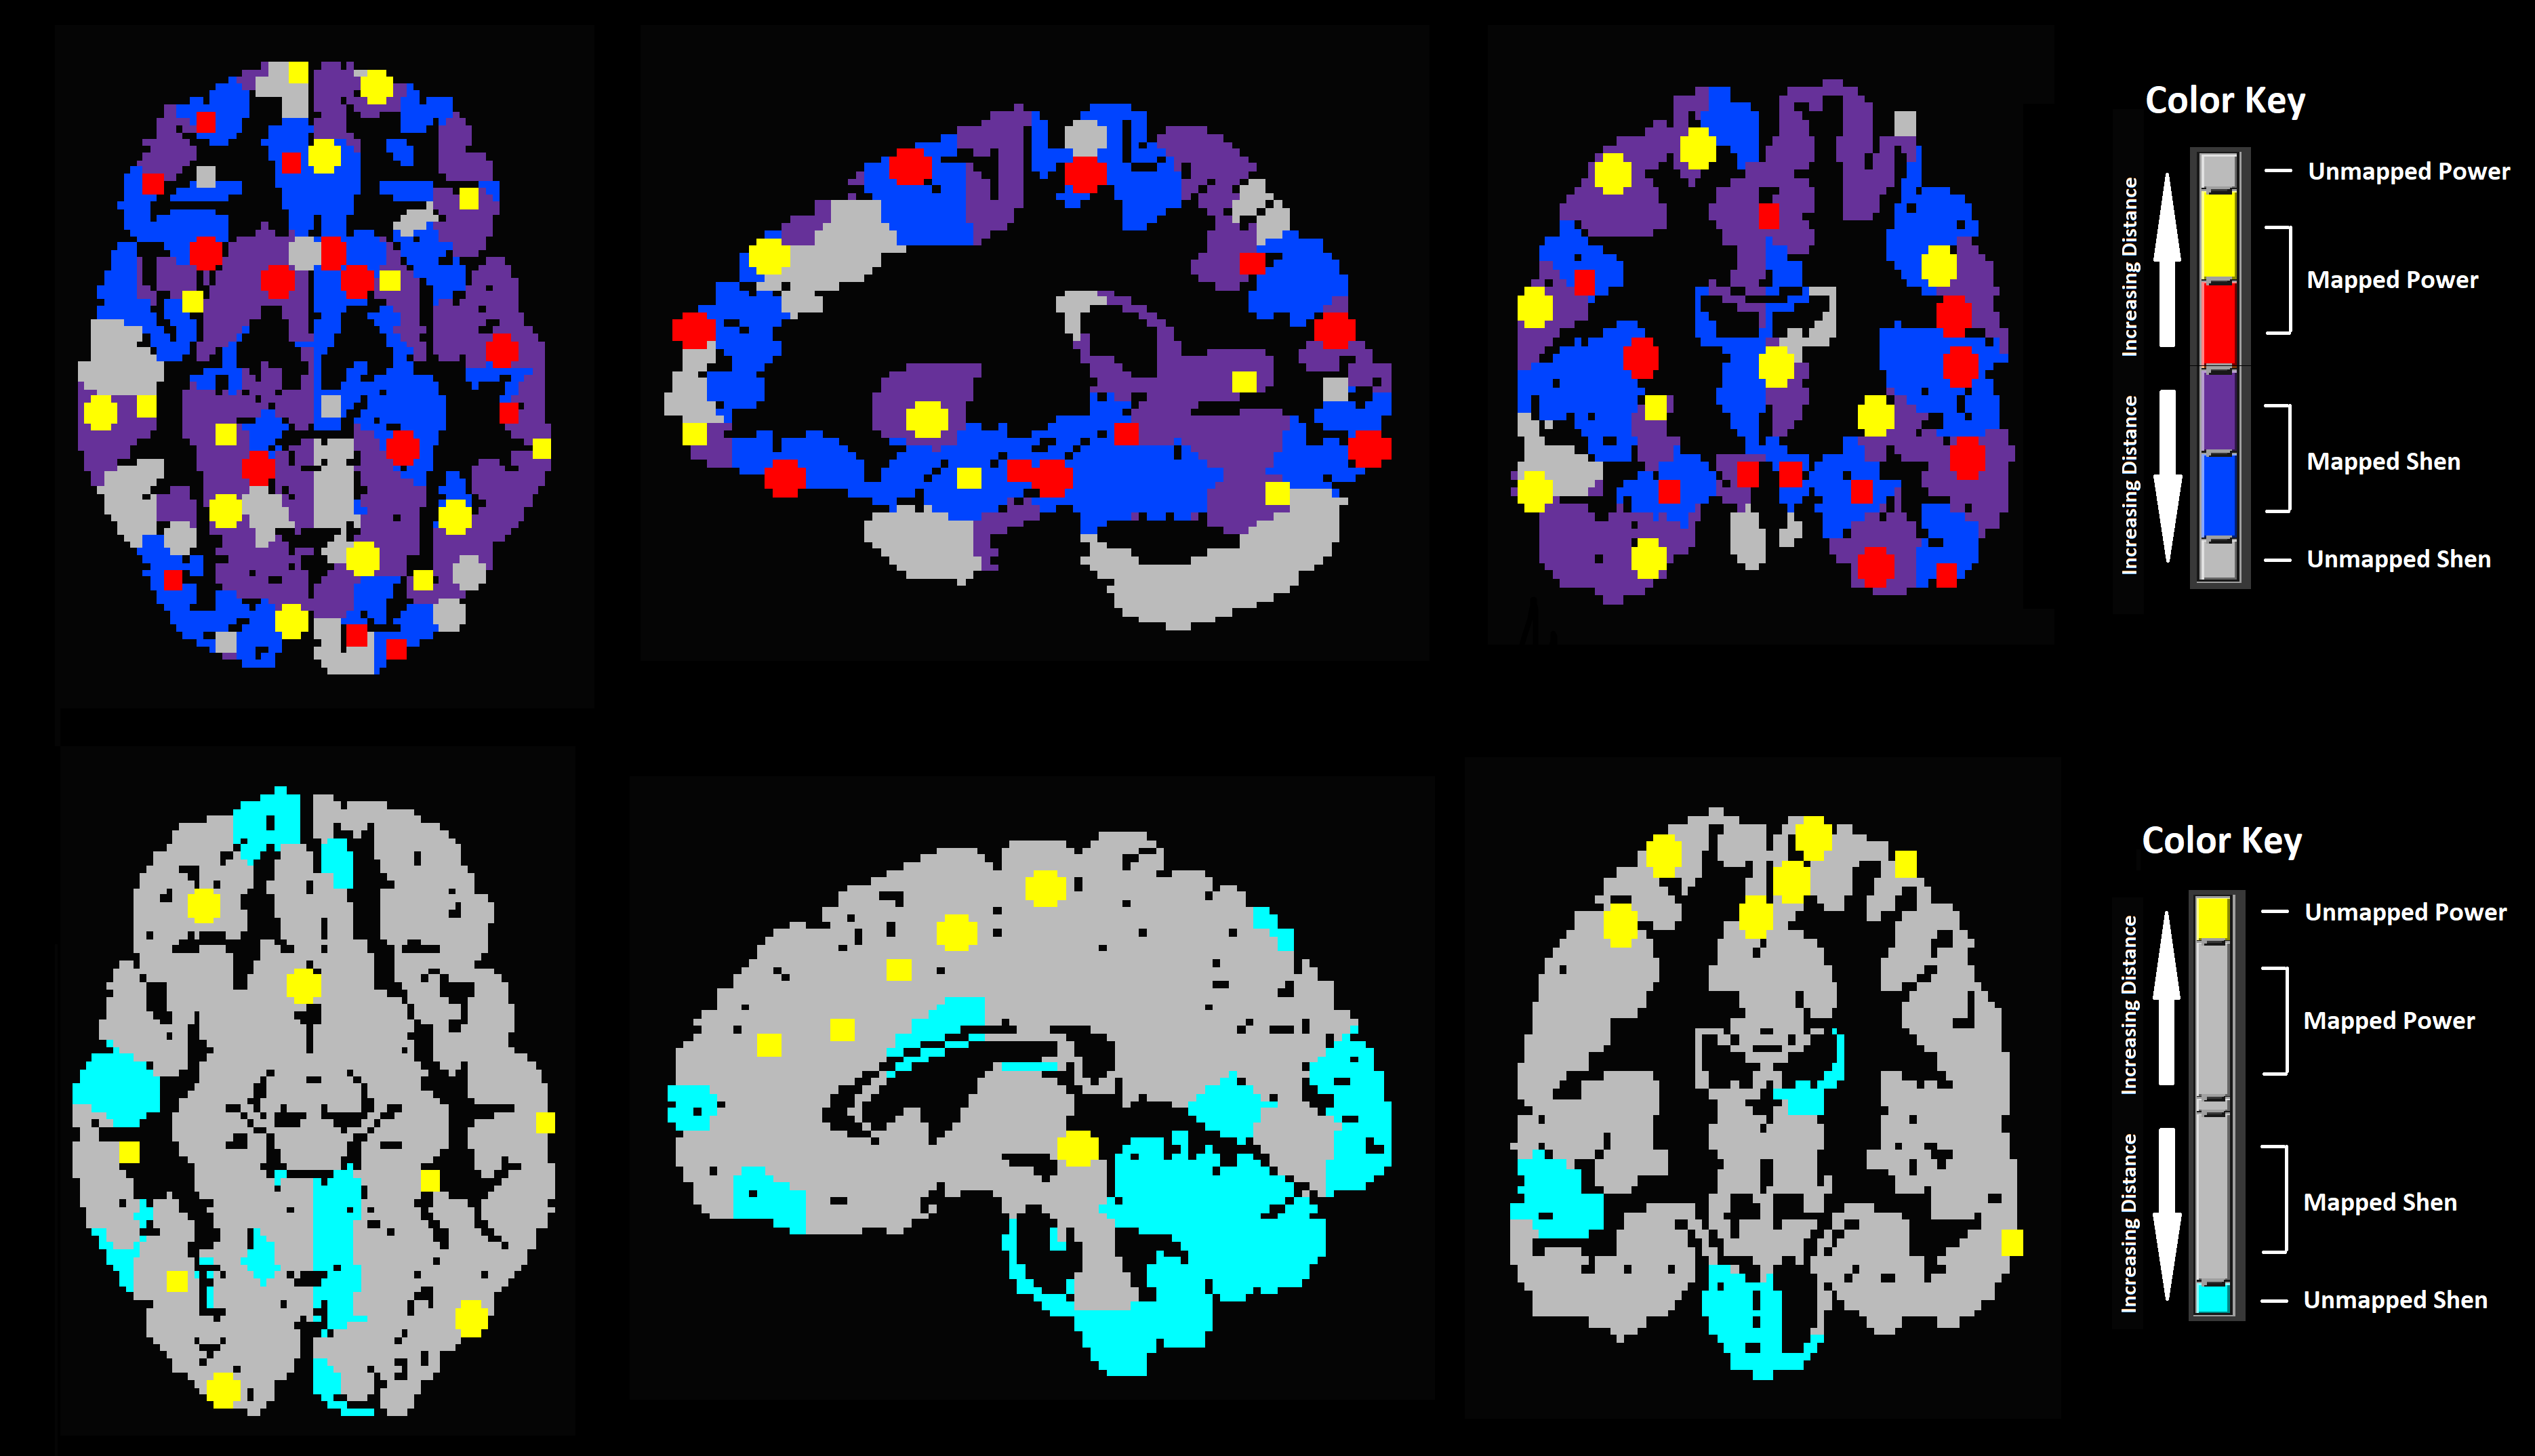
\includegraphics[width=1\textwidth,clip,trim=0cm 0cm 0cm 0.0cm]{mapped-unmapped-montage.png}
	\caption{Visualization of mapped and unmapped ROIs from Power and Shen ROIs, respectively, from Assignment Problem solution. Two-dimensional slices from each atlas are overlaid on top of each other. The upper slices highlight the mapped ROIs from each atlas. The lower slices highlight the unmapped ROIs from each atlas.}\label{fig:power_shen_mapped-unmapped}
\end{figure}

Mapped ROIs are an indication of informational and spatial similarity shared by both atlases. Subject data that is derived from the mapped ROIs are highly correlated because each ROI pair shares voxels from which ROI time series are created. Unmapped ROIs in a single atlas may or may not intersect one of the mapped ROIs in another atlas. These unmapped ROIs indicate the most unique aspects of each atlas relative to one another. Hence, unmapped ROIs should be considered for inclusion in a customized atlas if determined to be important for predicting the outcome.

\subsection{Power and Shen atlas ROIs relevant to MDD}
We used GWAK to determine the value of $k$ that maximized the NPDR standardized beta coefficient $\beta_a$ (Eq.~\ref{eq:glm_roi}) for each atlas ROI. Important mapped (Table~\ref{tab:mapped-power-tab}) and unmapped (Table~\ref{tab:unmapped-power-tab}) Power ROIs correspond to several brain regions with known associations with MDD. The highest ranked Power ROI is designated as 89 with respect to that atlas, which is in the right precuneus brain region in the dorsal default mode network (DMN). The precuneus in general, and the right precuneues in particular, has previously been associated with MDD~\cite{cheng2018,dutta2019,liu2017}. 

Aside from the left middle temporal gyrus, each of the important mapped Power ROI brain regions (Table~\ref{tab:mapped-power-tab}) has been identified in several other studies regarding MDD patients versus healthy controls: left inferior temporal gyrus~\cite{ramezani2014,rolls2017}, left parahippocampal gyrus~\cite{ramezani2014,zeng2012}, right middle frontal gyrus~\cite{reynolds2014,fitzgerald2008}, left cingulate gyrus~\cite{hamani2011,mclaren2016}, right superior frontal gyrus~\cite{tao2013,salvadore2011}, right supramarginal gyrus~\cite{peng2015,tu2018}, right orbital gyrus~\cite{rolls2017,yan2019}, right medial frontal gyrus~\cite{lemogne2009,tao2013}, right caudate head~\cite{pizzagalli2009,bluhm2009}, right inferior frontal gyrus~\cite{tao2013,tu2018}, right superior temporal gyrus~\cite{pan2015}, left lingual gyrus~\cite{jung2014,couvy-duchesne2018}, and right cuneus~\cite{bai2018,guo2014}.

Similar to the collection of important mapped Power ROIs (Table~\ref{tab:mapped-power-tab}), each important unmapped Power ROI brain region, other than the left middle temporal gyrus, has been identified in other studies that compared MDD patients with healthy controls: right middle temporal gyrus~\cite{rolls2017}, right inferior parietal lobule~\cite{cooney2010}, left medial frontal gyrus~\cite{fitzgerald2008}, left insula~\cite{schmaal2017,li2017}, right postcentral gyrus~\cite{schmaal2017}, and left cingulate gyrus~\cite{mclaren2016,hamani2011}.

NPDR-detected functional networks relevant to MDD have all been previously associated with the disorder: dorsal default mode network (DMN)~\cite{hamilton2015,yan2019-2,dutta2019,lois2016,guo2014-2,menon2011}, left executive control network (LECN)~\cite{zhao2019,ellard2018,liu2012}, right executive control network (RECN)~\cite{zhao2019,ellard2018,liu2012}, language network~\cite{schultz2018,wu2017}, primary visual network~\cite{wu2017}, sensorimotor network~\cite{wu2017,zhi2018,zhuo2017}, and anterior salience network~\cite{sikora2017,wang2016}.

Nearly every Shen atlas ROI intersects multiple brain regions, as determined by Shen ROI intersection with Power ROIs that have unique brain region associations. We highlighted brain regions corresponding to mapped and unmapped important Shen ROIs (Tables~\ref{tab:mapped-shen-tab}-\ref{tab:unmapped-shen-tab}) that were not detected as important with respect to the Power atlas. Some of the highlighted brain regions for significant ROIs may not actually be relevant because many of the detected Shen ROIs intersect important Power ROIs. Some of the brain regions intersected by important Shen ROIs, such as left culmen, left declive, right lingual gyrus, locus coeruleus, right declive, right parahippocampal gyrus, left inferior frontal gyrus, right uvula, left superior temporal gyrus, left precentral gyrus, left inferior parietal lobule, right superior parietal lobule, left middle occipital gyrus, left inferior occipital gyrus, right paracentral lobule, and left middle frontal, are the only brain regions associated with the particular Shen ROI. Almost all of these regions are relevant to MDD, but more investigation must be done to determine if the corresponding Shen ROI is important due to the incorporation of these brain regions or if significance is related to another associated brain region. For example, the most significant Shen ROI is labeled 243 (Table~\ref{tab:mapped-shen-tab}), which intersects the left inferior temporal gyrus, the left parahippocampal gyrus, and the left fusiform gyrus. The left inferior temporal gyrus and left parahippocampal gyrus are the brain regions that contain ROIs 4 and 77 in the Power atlas (Table~\ref{tab:mapped-power-tab}), which are among the top 3 significant Power ROIs. This confounds our ability to label the left fusiform gyrus as important with respect to these two atlases, however, this brain region has been associated with MDD in other studies~\cite{iwabuchi2015,kroes2011}. 

Nearly all brain regions intersected by important Shen ROIs, but not containing any important Power ROIs, are all associated with MDD in other studies: left fusiform gyrus~\cite{iwabuchi2015,kroes2011}, right insula~\cite{avery2014,iwabuchi2014}, right lentiform nucleus~\cite{lui2009,helm2018}, left superior frontal gyrus~\cite{fitzgerald2008,tao2013}, left culmen~\cite{su2014,yamamura2016}, left declive~\cite{su2014,lin2012}, right lingual gyrus~\cite{couvy-duchesne2018,jung2014}, left postcentral gyrus~\cite{zhang2019,schmaal2017}, left precentral gyrus~\cite{tsujii2017,shen2015}, right inferior occipital gyrus~\cite{grieve2013,peterson2009}, locus coeruleus~\cite{wang2017,seki2019}, right declive~\cite{su2014,lin2012}, right fusiform gyrus~\cite{kroes2011,lin2017}, right inferior temporal gyrus~\cite{ramezani2014}, right parahippocampal gyrus~\cite{zamoscik2014,kalsi2017}, left paracentral lobule~\cite{rolls2017,sinha2019}, left inferior frontal gyrus~\cite{tao2013,xu2019}, right uvula~\cite{deldonno2018}, left inferior occipital gyrus~\cite{peterson2009}, left middle occipital gyrus~\cite{ma2019,teng2018}, left inferior parietal lobule~\cite{tu2018,teng2018}, right superior parietal lobule~\cite{zhang2017,chen2015}, right paracentral lobule, right angular gyrus, left cuneus, left middle frontal gyrus, right precentral gyrus, left uncus, right middle occipital gyrus.

\begin{table}[h!]
	\centering
	\caption{Standardized beta coefficients, P values, and brain regions for important mapped Power atlas ROIs.}\label{tab:mapped-power-tab}
	\begin{tabular}[h!]{ccccc}\toprule
		\textbf{ROI} & \bm{$\beta_a$} & \textbf{P Value} & \textbf{Brain Region} & \textbf{Func. Network} \\ \midrule
		89 & 5.6464 & 5.87e-06 & Right Precuneus & Dorsal DMN \\
		4 & 5.3591 & 2.49e-05 & Left Inferior Temporal Gyrus & LECN \\
		77 & 5.1431 & 8.35e-05 & Left Parahippocampal Gyrus & Dorsal DMN \\
		181 & 4.7650 & 4.28e-04 & Right Middle Frontal Gyrus & RECN \\
		59 & 4.6523 & 7.55e-04 & Left Cingulate Gyrus & Anterior Salience \\
		180 & 4.6062 & 8.86e-04 & Right Superior Frontal Gyrus & NA \\
		204 & 4.5755 & 1.04e-03 & Right Supramarginal Gyrus & RECN \\
		5 & 4.5654 & 1.07e-03 & Right Orbital Gyrus & Dorsal DMN \\
		110 & 4.3227 & 3.08e-03 & Right Medial Frontal Gyrus & Dorsal DMN \\
		129 & 4.2442 & 4.23e-03 & Left Middle Temporal Gyrus & Language \\
		76 & 4.2390 & 4.60e-03 & Right Medial Frontal Gyrus & Dorsal DMN \\
		270 & 4.1885 & 5.29e-03 & Right Caudate Head & NA \\
		85 & 3.8958 & 1.72e-02 & Right Inferior Frontal Gyrus & NA \\
		82 & 3.8729 & 1.88e-02 & Right Superior Temporal Gyrus & NA \\
		160 & 3.7058 & 3.54e-02 & Left Lingual Gyrus & Primary Visual\\
		145 & 3.6940 & 3.76e-02 & Right Cuneus & Primary Visual \\ \bottomrule
	\end{tabular}
\end{table}

\begin{table}[h!]
	\centering
    \caption{Standardized beta coefficients, P values, and brain regions for important unmapped Power atlas ROIs.}\label{tab:unmapped-power-tab}
	\begin{tabular}[h!]{ccccc}\toprule
		\textbf{ROI} & \bm{$\beta_a$} & \textbf{P Value} & \textbf{Brain Region} & \textbf{Func. Network} \\ \midrule
		83 & 5.6804 & 4.92e-06 & Left Middle Temporal Gyrus & LECN \\
		128 & 4.9002 & 2.32e-04 & Right Middle Temporal Gyrus & NA \\
		192 & 4.0946 & 7.95e-03 & Right Inferior Parietal Lobule & RECN \\
		35 & 4.0692 & 8.59e-03 & Left Medial Frontal Gyrus & Sensorimotor \\
		73 & 4.0154 & 1.08e-02 & Left Insula & NA \\
		36 & 3.8673 & 2.19e-02 & Right Postcentral Gyrus & Sensorimotor \\
		213 & 3.6807 & 4.52e-02 & Left Cingulate Gyrus & Anterior Salience \\ \bottomrule
	\end{tabular}
\end{table}

\begin{longtable}[c]{cccp{3.2in}}
	\caption{Standardized beta coefficients, P values, and brain regions for important mapped Shen atlas ROIs. Brain regions were assigned to each Shen ROI based on overlap with known Power ROI brain regions. Brain regions for Shen ROIs that did not overlap any Power ROIs were assigned NA. Brain regions that did not show up in the list of important Power ROIs (Tables~\ref{tab:mapped-power-tab}-\ref{tab:unmapped-power-tab}) are highlighted.}\label{tab:mapped-shen-tab}\\ \toprule
	
	\multicolumn{1}{c}{\textbf{ROI}} & \multicolumn{1}{c}{\bm{$\beta_a$}} & \multicolumn{1}{c}{\textbf{P Value}} & \multicolumn{1}{c}{\textbf{Brain Region}} \\ \bottomrule 
	\endfirsthead
	
	\multicolumn{4}{c}%
	{{\bfseries \tablename\ \thetable{} -- continued from previous page}} \\
	\hline \multicolumn{1}{c}{\textbf{ROI}} & \multicolumn{1}{c}{\bm{$\beta_a$}} & \multicolumn{1}{c}{\textbf{P Value}} & \multicolumn{1}{c}{\textbf{Brain Region}} \\ \bottomrule
	\endhead
	
	\midrule \multicolumn{4}{r}{\textbf{Continued on next page}} \\ \bottomrule
	\endfoot
	
	\bottomrule
	\endlastfoot
	243 & 13.4157 & 2.41e-38 & Left Inferior Temporal Gyrus, Left Parahippocampal Gyrus, \hl{Left Fusiform Gyrus} \\
	99 & 13.1216 & 1.09e-36 & Right Middle Temporal Gyrus, \hl{Right Insula}, \hl{Right Lentiform Nucleus} \\
	5 & 11.6413 & 7.29e-29 & Right Postcentral Gyrus, Right Inferior Parietal Lobule \\
	29 & 11.3464 & 2.06e-27 & Right Postcentral Gyrus \\
	277 & 9.5110 & 3.64e-19 & \hl{Left Superior Frontal Gyrus}, Left Medial Frontal Gyrus \\
	178 & 9.1192 & 1.40e-17 & \hl{Left Culmen}, \hl{Left Declive} \\
	127 & 8.5795 & 1.66e-15 & \hl{Right Lingual Gyrus} \\
	105 & 7.4976 & 1.03e-11 & Right Medial Frontal Gyrus, Right Middle Frontal Gyrus, Right Superior Frontal Gyrus\\
	262 & 7.4889 & 1.10e-11 & \hl{Left Postcentral Gyrus}, \hl{Left Precentral Gyrus}, Left Medial Frontal Gyrus \\
	96 & 7.0001 & 3.94e-10 & \hl{Right Inferior Occipital Gyrus}, \hl{Right Lingual Gyrus} \\
	239 & 6.9550 & 5.39e-10 & \hl{Locus Coeruleus} \\
	104 & 6.8045 & 1.54e-09 & \hl{Right Declive} \\
	217 & 6.6554 & 4.25e-09 & Left Parahippocampal Gyrus, \hl{Left Fusiform Gyrus} \\
	238 & 6.4225 & 2.00e-08 & Left Middle Temporal Gyrus \\
	83 & 6.3879 & 2.55e-08 & Right Superior Temporal Gyrus \\
	57 & 6.3269 & 3.71e-08 & Right Inferior Parietal Lobule, Right Postcentral Gyrus \\
	7 & 6.2803 & 5.01e-08 & Right Middle Frontal Gyrus, \hl{Right Precentral Gyrus} \\
	12 & 6.2222 & 7.29e-08 & \hl{Right Lingual Gyrus}, Right Cuneus \\
	32 & 6.1985 & 8.42e-08 & Right Precentral Gyrus, Right Postcentral Gyrus \\
	102 & 6.1316 & 1.28e-07 & \hl{Right Inferior Occipital Gyrus}, Right Middle Occipital Gyrus \\
	19 & 6.0343 & 2.34e-07 & \hl{Right Fusiform Gyrus}, Right Middle Temporal Gyrus, \hl{Right Inferior Temporal Gyrus} \\
	21 & 6.0037 & 2.83e-07 & \hl{Right Cingulate Gyrus}, Right Precuneus \\
	202 & 5.7008 & 1.74e-06 & \hl{Left Declive}, \hl{Left Culmen} \\
	136 & 5.6781 & 1.98e-06 & \hl{Right Parahippocampal Gyrus} \\
	253 & 5.5841 & 3.40e-06 & Right Medial Frontal Gyrus, Left Medial Frontal Gyrus, \hl{Left Paracentral Lobule} \\
	113 & 5.4798 & 6.17e-06 & \hl{Right Culmen}, \hl{Right Parahippocampal Gyrus} \\
	271 & 5.3379 & 1.41e-05 & Left Medial Frontal Gyrus \\
	215 & 5.2170 & 2.86e-05 & \hl{Left Inferior Frontal Gyrus} \\
	130 & 5.1917 & 2.99e-05 & \hl{Right Uvula} \\
	257 & 5.0391 & 6.68e-05 & Left Lingual Gyrus, \hl{Left Inferior Occipital Gyrus}, \hl{Left Middle Occipital Gyrus} \\
	237 & 5.0153 & 7.61e-05 & \hl{Left Superior Temporal Gyrus}, \hl{Left Precentral Gyrus} \\
	245 & 5.0136 & 7.68e-05 & \hl{Left Superior Temporal Gyrus}, \hl{Left Inferior Parietal Lobule} \\
	80 & 4.7380 & 3.07e-04 & \hl{Right Superior Parietal Lobule}, Right Precuneus \\
	247 & 4.7039 & 3.63e-04 & \hl{Left Middle Occipital Gyrus}, \hl{Left Inferior Occipital Gyrus} \\
	55 & 4.5641 & 7.10e-04 & \hl{Right Paracentral Lobule}, Left Cingulate Gyrus, Right Medial Frontal Gyrus \\
	8 & 4.5240 & 8.59e-04 & Right Postcentral Gyrus \\
	45 & 4.4630 & 1.14e-03 & Right Medial Frontal Gyrus, Right Postcentral Gyrus \\
	24 & 4.4623 & 1.15e-03 & Right Supramarginal Gyrus, \hl{Right Angular Gyrus}, Right Inferior Parietal Lobule \\
	84 & 4.4571 & 1.18e-03 & \hl{Left Cuneus}, Right Precuneus, Right Cuneus \\
	121 & 4.3935 & 1.58e-03 & \hl{Right Lingual Gyrus} \\
	206 & 4.1698 & 4.32e-03 & \hl{Left Inferior Frontal Gyrus} \\
	38 & 4.1499 & 4.83e-03 & \hl{Right Uvula} \\
	193 & 4.1029 & 5.74e-03 & \hl{Left Middle Frontal Gyrus} \\
	28 & 4.0366 & 7.66e-03 & Right Postcentral Gyrus, \hl{Right Precentral Gyrus} \\
	213 & 3.9603 & 1.05e-02 & \hl{Left Uncus}, Left Parahippocampal Gyrus \\
	147 & 3.8788 & 1.48e-02 & \hl{Left Middle Occipital Gyrus}, Left Middle Temporal Gyrus \\
	87 & 3.8019 & 2.01e-02 & \hl{Right Fusiform Gyrus}, Right Middle Temporal Gyrus, \hl{Right Middle Occipital Gyrus} \\
	218 & 3.6315 & 3.96e-02 & \hl{Left Precentral Gyrus} \\
	103 & 3.5907 & 4.64e-02 & Right Inferior Frontal Gyrus \\
\end{longtable}

\begin{table}[h!]
	\centering
	\caption{Standardized beta coefficients, P values, and brain regions for important unmapped Shen atlas ROIs. Brain regions were assigned to each Shen ROI based on overlap with known Power ROI brain regions. Brain regions for Shen ROIs that did not overlap any Power ROIs were assigned NA.}\label{tab:unmapped-shen-tab}
\begin{tabular}[h!]{cccc}\toprule
	\textbf{ROI} & \bm{$\beta_a$} & \textbf{P Value} & \textbf{Brain Region} \\ \midrule
	49 & 9.5173 & 3.40e-19 & NA \\
	3 & 9.3489 & 1.67e-18 & Right Medial Frontal Gyrus \\
	76 & 9.0332 & 3.04e-17 & NA \\
	79 & 9.0313 & 3.08e-17 & NA \\
	175 & 8.4150 & 6.68e-15 & \hl{Right Declive} \\
	219 & 7.8334 & 7.68e-13 & NA\\
	35 & 7.7575 & 1.39e-12 & Right Middle Temporal Gyrus\\
	231 & 7.5458 & 7.13e-12 & \hl{Left Declive}, \hl{Right Declive}, Left Lingual Gyrus\\
	174 & 7.5352 & 7.72e-12 & NA \\
	256 & 7.3053 & 4.32e-11 & \hl{Left Declive} \\
	141 & 7.2127 & 8.50e-11 & NA \\
	13 & 6.2918 & 4.65e-08 & NA \\
	158 & 6.2916 & 4.67e-08 & NA \\
	196 & 5.9340 & 4.33e-07 & NA \\
	126 & 4.9343 & 1.15e-04 & \hl{Right Uvula} \\
	31 & 4.8789 & 1.52e-04 & NA \\
	70 & 4.8009 & 2.25e-04 & NA \\
	115 & 4.6691 & 4.33e-04 & \hl{Locus Coeruleus} \\ \bottomrule
\end{tabular}
\end{table}

\section{Discussion}

\bibliographystyle{unsrt}
\bibliography{BoD}   % name of bib file
\end{document}
